%------------------------------------------------
%	PACKAGES AND THEMES
%------------------------------------------------

% this is a 4:3 layout.
\documentclass{beamer}
% for 16:9 use this command:
% \documentclass[aspectratio=169]{beamer}

\mode<presentation> {
\usetheme{metropolis}
\setbeamertemplate{caption}[numbered]
\setbeamertemplate{navigation symbols}{} % hide navigation symbols
}

\usepackage{graphicx} % images
\usepackage{algorithm2e}
\usepackage{mathtools}
\DeclarePairedDelimiter{\ceil}{\lceil}{\rceil}
\usepackage{algpseudocode}
\usepackage{booktabs} % allows the use of \toprule, \midrule and \bottomrule in tables
\usepackage[ngerman]{babel}
\usepackage[utf8]{inputenc}
\usepackage[T1]{fontenc}
\usepackage{mathtools}
\usepackage{xcolor}
\usepackage{listings} % code
\usepackage{pgf,tikz} % drawing
\usepackage{pifont} % new symbols
\usepackage{hyperref} % pretty links
% \usepackage{algorithmicx}
% \usepackage{algpseudocode}
% \usepackage[linesnumbered,ruled]{algorithm2e}

\usepackage{lmodern}
\usepackage{subcaption}
\usepackage{textcomp}
% \usepackage{array}
% \usepackage{longtable}
% \usepackage{verbatim}
%\usepackage{tabularx}
\captionsetup[figure]{font=footnotesize}

\usepackage{amsmath}
\usepackage{amssymb}
\usepackage{amsthm}
% \usepackage{comment}
% \usepackage{enumitem}
% \usepackage[binary-units=true]{siunitx}
% \usepackage{thmtools}
\usepackage{csquotes}
\usepackage{tikz}
\usepackage{float}
\usetikzlibrary{automata,positioning}

% color settings for links
\hypersetup{
    colorlinks=true,
    urlcolor=blue,
    linkcolor=black,
    citecolor=green!50!black
}

\definecolor{mygreen}{RGB}{1,135,1}

\newcommand{\cmark}{\ding{51}}  % checkmark
\newcommand{\xmark}{\ding{55}}  % xmark
\newcommand\scalemath[2]{\scalebox{#1}{\mbox{\ensuremath{\displaystyle #2}}}}

% \useoutertheme{miniframes} % navigation design
\useinnertheme{circles} % use non shiny circles (itemize, etc.)

% Main slide colors
% dunkel, hell, mittel
% \definecolor{pale}{RGB}{232, 236, 237}
% \definecolor{prim}{RGB}{53, 109, 120}
% \definecolor{sec}{RGB}{104, 170, 183}
% \definecolor{tert}{RGB}{109, 155, 168}
% \definecolor{quat}{RGB}{9, 59, 68}

\definecolor{pale}{RGB}{232, 236, 237}
% \definecolor{prim}{RGB}{153, 194, 173}
% good: \definecolor{prim}{RGB}{27, 33, 42}
\definecolor{prim}{RGB}{32, 43, 50}
\definecolor{sec}{RGB}{217, 232, 224}
\definecolor{tert}{RGB}{0, 82, 41}
% save
\definecolor{quat}{RGB}{0, 82, 41}

\setbeamercolor{palette primary}{bg=prim,fg=pale}
\setbeamercolor{palette secondary}{bg=sec,fg=pale}
\setbeamercolor{palette tertiary}{bg=tert,fg=pale}
\setbeamercolor{palette quaternary}{bg=quat,fg=pale}
\setbeamercolor{structure}{fg=prim} % itemize, enumerate, etc
\setbeamercolor{section in toc}{fg=prim} % TOC sections

% Block colors
\definecolor{example_color}{RGB}{93, 137, 98}
\definecolor{alert_color}{RGB}{175, 79, 72}

\setbeamercolor{normal text}{fg=prim!20!black,bg=pale!25!white}
\setbeamercolor{alerted text}{fg=alert_color!25!black}
\setbeamercolor{example text}{fg=example_color!25!black}

\setbeamercolor{block title example}{fg=white,bg=example_color}
\setbeamercolor{block body example}{fg=black,bg=example_color!10!white}
\setbeamercolor{block title alerted}{fg=white,bg=alert_color}
\setbeamercolor{block body alerted}{fg=black,bg=alert_color!10!white}

% Override palette coloring
\setbeamercolor{subsection in head/foot}{bg=quat,fg=pale}

\setbeamertemplate{frametitle}{%
    \nointerlineskip%

    \begin{beamercolorbox}[wd=\paperwidth,ht=2.5ex,dp=1ex]{frametitle}
        \hspace*{1ex}\insertframetitle%
        \ifx\insertframesubtitle@empty\else%
        {~\tiny\textcolor{quat!35!black}{\insertframesubtitle}}%
        \fi%
    \end{beamercolorbox}%
}

% math-command for bigger norm
\newcommand\norm[1]{\left\lVert#1\right\rVert}

% use this to include other files
% in this case style definitions for code
% alternative: \include{dateiname}
\lstdefinestyle{latex}{
    language=[LaTeX]TeX,
    inputencoding=utf8,
    basicstyle=\ttfamily,
    keywordstyle=\color{blue!60!black}, % use 60 percent blue and 40 black
    commentstyle=\color{cyan!60!black},
    tabsize=2,
    emph={document,itemize,enumerate,center,tabular,table,
    figure,wrapfigure,minipage,columns,align,bmatrix,
    lstlisting,beamer,frame,tikzpicture},
    emphstyle=\color{magenta!60!black},
    morekeywords={lstset,includegraphics,theenumi,labelitemi,column,color,url,href}
}

\lstdefinestyle{inline_latex}{
    language=[LaTeX]TeX,
    inputencoding=utf8,
    basicstyle=\ttfamily,
    resetmargins= true,
    belowcaptionskip=0pt,
    aboveskip=0pt,
    belowskip=0pt,
    keywordstyle=\color{blue!60!black},
    commentstyle=\color{cyan!60!black},
    emph={document,itemize,enumerate,center,tabular,table,
    figure,wrapfigure,minipage,columns,align,bmatrix,
    lstlisting,beamer,frame,tikzpicture,Parameter},
    emphstyle=\color{magenta!60!black},
    morekeywords={lstset,includegraphics,theenumi,labelitemi,column,color,url,href,Befehlsname}
}

\lstdefinestyle{cpp}{
    language=C++,
    basicstyle=\ttfamily,
    keywordstyle=\color{blue!90!black},
    stringstyle=\color{magenta!60!black},
    commentstyle=\color{green!35!black},
    morecomment=[l][\color{gray!60!black}]{\#},
    tabsize=2
}

\lstdefinestyle{empty}{
    basicstyle=\rmfamily,
    keywordstyle=\bfseries,
    commentstyle=\color{black}\itshape
}

\lstset{style=latex}

%------------------------------------------------
%	TITLE PAGE
%------------------------------------------------

\selectlanguage{ngerman}
\title[]{Single Vehicle Problems \textsc{PTP} / \textsc{PCTSP} / \textsc{OP}}

\author{Tim Bohne, Thomas Klein}
\institute[]
{
\textit{Master-Projektgruppe - Team Orienteering Problems für individuelle Touristenrouten}
\medskip
}
\date{\today}

% make slide at the beginnig of each section
\AtBeginSection[]{
{\setbeamercolor{background canvas}{bg=white}}}

% where images are locatied
\graphicspath{{./images/}}

\begin{document}

\begin{frame}[plain] % plain slides dont have navigation bars etc.
\titlepage % Print the title page as the first slide
\end{frame}

\begin{frame}
\frametitle{Übersicht} % table of contents slide
\tableofcontents
\end{frame}

%------------------------------------------------
\section{Single Vehicle Routing Problems with Profits}
%------------------------------------------------

\begin{frame}
  \frametitle{Single Vehicle Routing Problems with Profits}
  \textbf{Input:}
  \begin{itemize}
    \item $G = (N, A)$
    \item \textbf{Knoten} $i \in N = \{1, ..., |N|\}$ mit $P_i \geq 0$
    \item \textbf{Startknoten} $1$, \textbf{Endknoten} $|N|$ ($P_1 = P_{|N|} = 0)$
    \item \textbf{Kosten} $t_{ij} \in A, t_{ij} \geq 0$ zwischen Knoten $i$ und $j$
  \end{itemize}
\end{frame}

\begin{frame}
\frametitle{Single Vehicle Routing Problems with Profits}
\begin{itemize}
  \item \textbf{3 Varianten}: \textsc{PTP}, \textsc{PCTSP}, \textsc{OP}
  \item \textbf{Unterschied}: Modellierung von \textit{profit} und \textit{travel costs}
  \item \textbf{Abgrenzung zum \textsc{TSP}}:\newline Es wird basierend auf der betrachteten
  Zielfunktion nur eine Teilmenge der Knoten besucht
\end{itemize}
\end{frame}

%------------------------------------------------
\section{Profitable Tour Problem (\textsc{PTP})}
%------------------------------------------------

\begin{frame}
\frametitle{Profitable Tour Problem (\textsc{PTP})}
\begin{itemize}
  \item Zielfunktion kombiniert \textit{profit} und \textit{travel costs}:\newline
  $max$ (\textit{profit} $-$ \textit{travel costs})
  \item \textbf{Ziel}: Bestimme Route, die bei Knoten $1$ startet und bei Knoten $|N|$ endet, die eine Teilmenge von $N$
  enthält und die Differenz aus Gesamtprofit und Gesamtkosten maximiert
  \item Route einer optimalen Lösung entspricht \textsc{TSP}-Route für die ausgewählten Knoten
  \item NP-schwer
\end{itemize}
\end{frame}

\begin{frame}
  \frametitle{Profitable Tour Problem (\textsc{PTP})}
  \scalebox{0.7}{\parbox{\linewidth}{%
  \begin{itemize}
    \item $x_{ij} = 1$: Nach $i$ wird $j$ besucht
    \item $u_i$: Position von $i$ in der Route\newline
  \end{itemize}
  \begin{gather}
    \boldsymbol{max} \quad \sum_{i = 1}^{|N| - 1} \sum_{j = 2}^{|N|} (P_i x_{ij} - t_{ij} x_{ij}) \\
    \boldsymbol{s.t.} \quad \sum_{j = 2}^{|N|} x_{1j} = \sum_{i = 1}^{|N| - 1} x_{i|N|} = 1 \\
    \sum_{i = 1}^{|N| - 1} x_{ik} = \sum_{j = 2}^{|N|} x_{kj} \leq 1 \quad \forall k = 2, ..., (|N| - 1) \\
    2 \leq u_i \leq |N| \quad \forall i = 2, ..., |N| \\
    u_i - u_j + 1 \leq (|N| - 1)(1 - x_{ij}) \quad \forall i, j = 2, ..., |N| \\
    x_{ij} \in \{0, 1\}
  \end{gather}}}
\end{frame}

\begin{frame}
  \frametitle{Subtour Elimination}
  \begin{itemize}
    \item $N = \{1, 2, 3, 4, 5\}$
    \item Ohne NB $(4)$ und $(5)$ wären kombinierte Routen möglich, z.B.\newline
    $1-5-1$ und $2-3-4-2$
    \item Maßnahme: $x_{ij} = 1 \implies u_j \geq u_i + 1$
    \item Übersetzt in lineare NB: $u_i - u_j + 1 \leq (|N| - 1)(1 - x_{ij}) \quad \forall i, j = 2, ..., |N|$
    \item Test:
    \begin{itemize}
      \item $x_{ij} = 1: \quad u_i + 1 \leq u_j$ \checkmark
      \item $x_{ij} = 0: \quad u_i - u_j \leq |N| - 2$ \checkmark
    \end{itemize}
  \end{itemize}
\end{frame}

\begin{frame}
  \frametitle{Profitable Tour Problem (\textsc{PTP})}

      \begin{figure}[H]
      \begin{subfigure}[b]{0.45\textwidth}
      \centering
      \begin{tikzpicture}[scale=0.6, transform shape, node distance=1.75cm]
          \node[state] (A) [thick] {$\boldsymbol{A_{Dep}}$};
          \node[state] (B) [thick, above right = 1.75cm of A] {$\boldsymbol{B_5}$};
          \node[state] (E) [thick, below right = 1.75cm of A] {$\boldsymbol{E_4}$};
          \node[state] (C) [thick, right = 1.75cm of B] {$\boldsymbol{C_8}$};
          \node[state] (D) [thick, right = 1.75cm of E] {$\boldsymbol{D_1}$};

          \path
            (A) edge [thick, above left] node {$3$} (B)
            (A) edge [thick, above right, near end] node {$6$} (C)
            (A) edge [thick, above left, near start] node {$6$} (D)
            (A) edge [thick, below left] node {$3$} (E)
            (B) edge [thick, above] node {$4$} (C)
            (B) edge [thick, above right, near end] node {$5$} (D)
            (B) edge [thick, right] node {$3$} (E)
            (C) edge [thick, right] node {$3$} (D)
            (C) edge [thick, above left, near start] node {$5$} (E)
            (D) edge [thick, below] node {$4$} (E);
      \end{tikzpicture}
      \caption*{\textsc{Beispiel Netzwerk}}
      \end{subfigure}
      \hfill
      \begin{subfigure}[b]{0.45\textwidth}
      \centering
      \begin{tikzpicture}[scale=0.6, transform shape, node distance=1.75cm]
        \node[state] (A) [thick] {$\boldsymbol{A_{Dep}}$};
        \node[state] (B) [thick, above right = 1.75cm of A] {$\boldsymbol{B_5}$};
        \node[state] (E) [thick, below right = 1.75cm of A] {$\boldsymbol{E_4}$};
        \node[state] (C) [thick, right = 1.75cm of B] {$\boldsymbol{C_8}$};
        \node[state] (D) [thick, right = 1.75cm of E] {$\boldsymbol{D_1}$};

        \path
          (A) edge [thick, above left] node {$3$} (B)
          (A) edge [thick, below left] node {$3$} (E)
          (B) edge [thick, above] node {$4$} (C)
          (C) edge [thick, above left, near start] node {$5$} (E);
    \end{tikzpicture}
      \caption*{\textsc{optimale PTP Lösung}}
      \end{subfigure}
      \end{figure}
\end{frame}

%------------------------------------------------
\section{Prize-Collecting \textsc{TSP} (\textsc{PCTSP})}
%------------------------------------------------

\begin{frame}
\frametitle{Prize-Collecting \textsc{TSP} (\textsc{PCTSP})}
\begin{itemize}
  \item \textbf{Ziel}:\newline Bestimme Route, die eine Teilmenge aus $N$ mit Profit $\geq P_{min}$ enthält
  und die Gesamtkosten minimiert
  \item \textbf{Unterschied zum \textsc{TSP}}:
  \begin{itemize}
    \item Nicht alle Knoten müssen besucht werden
    \item Minimaler \textit{profit} muss erreicht werden
  \end{itemize}
  \item \textbf{Unterschied zum \textsc{PTP}}:
  \begin{itemize}
    \item \textit{profit} als Nebenbedingung, nicht als Teil der Zielfunktion
  \end{itemize}
  \item NP-schwer
\end{itemize}
\end{frame}

\begin{frame}
  \frametitle{Prize-Collecting \textsc{TSP} (\textsc{PCTSP})}
  \scalebox{0.7}{\parbox{\linewidth}{%
  \begin{itemize}
    \item $x_{ij} = 1$: Nach $i$ wird $j$ besucht
    \item $u_i$: Position von $i$ in der Route\newline
  \end{itemize}
  \begin{gather}
    \boldsymbol{min} \quad \sum_{i = 1}^{|N| - 1} \sum_{j = 2}^{|N|} t_{ij} x_{ij} \\
    \boldsymbol{s.t.} \quad \textcolor{olive}{\sum_{j = 2}^{|N|} x_{1j} = \sum_{i = 1}^{|N| - 1} x_{i|N|} = 1} \\
    \textcolor{olive}{\sum_{i = 1}^{|N| - 1} x_{ik} = \sum_{j = 2}^{|N|} x_{kj} \leq 1 \quad \forall k = 2, ..., (|N| - 1)} \\
    \sum_{i = 1}^{|N| - 1} \sum_{j = 2}^{|N|} P_i x_{ij} \geq P_{min} \\
    \textcolor{olive}{2 \leq u_i \leq |N| \quad \forall i = 2, ..., |N|} \\
    \textcolor{olive}{u_i - u_j + 1 \leq (|N| - 1)(1 - x_{ij}) \quad \forall i, j = 2, ..., |N|} \\
    x_{ij} \in \{0, 1\}
  \end{gather}}}
\end{frame}

\begin{frame}
  \frametitle{Prize-Collecting \textsc{TSP} (\textsc{PCTSP})}

  $P_{min} = 10$

      \begin{figure}[H]
      \begin{subfigure}[b]{0.45\textwidth}
      \centering
      \begin{tikzpicture}[scale=0.6, transform shape, node distance=1.75cm]
          \node[state] (A) [thick] {$\boldsymbol{A_{Dep}}$};
          \node[state] (B) [thick, above right = 1.75cm of A] {$\boldsymbol{B_5}$};
          \node[state] (E) [thick, below right = 1.75cm of A] {$\boldsymbol{E_4}$};
          \node[state] (C) [thick, right = 1.75cm of B] {$\boldsymbol{C_8}$};
          \node[state] (D) [thick, right = 1.75cm of E] {$\boldsymbol{D_1}$};

          \path
            (A) edge [thick, above left] node {$3$} (B)
            (A) edge [thick, above right, near end] node {$6$} (C)
            (A) edge [thick, above left, near start] node {$6$} (D)
            (A) edge [thick, below left] node {$3$} (E)
            (B) edge [thick, above] node {$4$} (C)
            (B) edge [thick, above right, near end] node {$5$} (D)
            (B) edge [thick, right] node {$3$} (E)
            (C) edge [thick, right] node {$3$} (D)
            (C) edge [thick, above left, near start] node {$5$} (E)
            (D) edge [thick, below] node {$4$} (E);
      \end{tikzpicture}
      \caption*{\textsc{Beispiel Netzwerk}}
      \end{subfigure}
      \hfill
      \begin{subfigure}[b]{0.45\textwidth}
      \centering
      \begin{tikzpicture}[scale=0.6, transform shape, node distance=1.75cm]
        \node[state] (A) [thick] {$\boldsymbol{A_{Dep}}$};
        \node[state] (B) [thick, above right = 1.75cm of A] {$\boldsymbol{B_5}$};
        \node[state] (E) [thick, below right = 1.75cm of A] {$\boldsymbol{E_4}$};
        \node[state] (C) [thick, right = 1.75cm of B] {$\boldsymbol{C_8}$};
        \node[state] (D) [thick, right = 1.75cm of E] {$\boldsymbol{D_1}$};

        \path
        (A) edge [thick, above left] node {$3$} (B)
        (A) edge [thick, above right, near end] node {$6$} (C)
        (B) edge [thick, above] node {$4$} (C);
    \end{tikzpicture}
      \caption*{\textsc{optimale \textsc{PCTSP} Lösung}}
      \end{subfigure}
      \end{figure}
\end{frame}

%------------------------------------------------
\section{Orienteering Problem (\textsc{OP})}
%------------------------------------------------

\begin{frame}
\frametitle{Orienteering Problem (\textsc{OP})}
\begin{itemize}
  \item \textbf{Ziel}:\newline Bestimme Route, die eine Teilmenge von $N$ enthält, durch $T_{max}$ limitiert ist
  und den Gesamtprofit maximiert
  \item Integriert Komplexität aus \textsc{Knapsack} und \textsc{TSP} \textrightarrow NP-schwer
  \item \textbf{Unterschied zum \textsc{TSP}}:
  \begin{itemize}
    \item Nicht alle Knoten müssen besucht werden
    \item Kosten sind nicht Teil der Zielfunktion
    \item Maximalkosten als Nebenbedingung
  \end{itemize}
  \item \textbf{Unterschied zum \textsc{PTP}}:
  \begin{itemize}
    \item Kosten als Nebenbedingung, nicht als Teil der Zielfunktion
  \end{itemize}
  \item \textbf{Unterschied zum \textsc{PCTSP}}:
  \begin{itemize}
    \item \textit{travel costs} und \textit{profit} tauschen \textquote{Rollen}
  \end{itemize}
\end{itemize}
\end{frame}

\begin{frame}
  \frametitle{Orienteering Problem (\textsc{OP})}
  \scalebox{0.7}{\parbox{\linewidth}{%
  \begin{itemize}
    \item $x_{ij} = 1$: Nach $i$ wird $j$ besucht
    \item $u_i$: Position von $i$ in der Route\newline
  \end{itemize}
  \begin{gather}
    \boldsymbol{max} \quad \sum_{i = 2}^{|N| - 1} \sum_{j = 2}^{|N|} P_i x_{ij} \\
    \boldsymbol{s.t.} \quad \textcolor{olive}{\sum_{j = 2}^{|N|} x_{1j} = \sum_{i = 1}^{|N| - 1} x_{i|N|} = 1} \\
    \textcolor{olive}{\sum_{i = 1}^{|N| - 1} x_{ik} = \sum_{j = 2}^{|N|} x_{kj} \leq 1 \quad \forall k = 2, ..., (|N| - 1)} \\
    \sum_{i = 1}^{|N| - 1} \sum_{j = 2}^{|N|} t_{ij} x_{ij} \leq T_{max} \\
    \textcolor{olive}{2 \leq u_i \leq |N| \quad \forall i = 2, ..., |N|} \\
    \textcolor{olive}{u_i - u_j + 1 \leq (|N| - 1)(1 - x_{ij}) \quad \forall i, j = 2, ..., |N|} \\
    x_{ij} \in \{0, 1\}
  \end{gather}}}
\end{frame}

\begin{frame}
  \frametitle{Orienteering Problem (\textsc{OP})}

  $T_{max} = 15$

      \begin{figure}[H]
      \begin{subfigure}[b]{0.45\textwidth}
      \centering
      \begin{tikzpicture}[scale=0.6, transform shape, node distance=1.75cm]
          \node[state] (A) [thick] {$\boldsymbol{A_{Dep}}$};
          \node[state] (B) [thick, above right = 1.75cm of A] {$\boldsymbol{B_5}$};
          \node[state] (E) [thick, below right = 1.75cm of A] {$\boldsymbol{E_4}$};
          \node[state] (C) [thick, right = 1.75cm of B] {$\boldsymbol{C_8}$};
          \node[state] (D) [thick, right = 1.75cm of E] {$\boldsymbol{D_1}$};
  
          \path          
            (A) edge [thick, above left] node {$3$} (B)
            (A) edge [thick, above right, near end] node {$6$} (C)
            (A) edge [thick, above left, near start] node {$6$} (D)
            (A) edge [thick, below left] node {$3$} (E)
            (B) edge [thick, above] node {$4$} (C)
            (B) edge [thick, above right, near end] node {$5$} (D)
            (B) edge [thick, right] node {$3$} (E)
            (C) edge [thick, right] node {$3$} (D)
            (C) edge [thick, above left, near start] node {$5$} (E)
            (D) edge [thick, below] node {$4$} (E);
      \end{tikzpicture}
      \caption*{\textsc{Beispiel Netzwerk}}
      \end{subfigure}
      \hfill
      \begin{subfigure}[b]{0.45\textwidth}
      \centering
      \begin{tikzpicture}[scale=0.6, transform shape, node distance=1.75cm]
        \node[state] (A) [thick] {$\boldsymbol{A_{Dep}}$};
        \node[state] (B) [thick, above right = 1.75cm of A] {$\boldsymbol{B_5}$};
        \node[state] (E) [thick, below right = 1.75cm of A] {$\boldsymbol{E_4}$};
        \node[state] (C) [thick, right = 1.75cm of B] {$\boldsymbol{C_8}$};
        \node[state] (D) [thick, right = 1.75cm of E] {$\boldsymbol{D_1}$};

        \path          
        (A) edge [thick, above left] node {$3$} (B)
            (A) edge [thick, below left] node {$3$} (E)
            (B) edge [thick, above] node {$4$} (C)
            (C) edge [thick, above left, near start] node {$5$} (E);
    \end{tikzpicture}
      \caption*{\textsc{optimale \textsc{OP} Lösung}}
      \end{subfigure}
      \end{figure}
\end{frame}

%------------------------------------------------
\section{Lösungsansätze für \textsc{OP}}
%------------------------------------------------

\begin{frame}
  \frametitle{OP Lösungsansätze}
  \textbf{exakt:}
  \begin{itemize}
    \item LP-Solver (CPLEX, Gurobi)
    \item Branch-and-Cut Algorithmus
  \end{itemize}
  \textbf{heuristisch:}
  \begin{itemize}
    \item Tsiligirides' S-/D- + RI-Algorithmus
    \item Center-of-Gravity Heuristik
    \item Lokale Suche / Metaheuristiken
  \end{itemize}
\end{frame}

\begin{frame}
  \frametitle{Tsiligirides' S-Algorithmus}
  \begin{itemize}
    \item Verwendet Monte-Carlo-Verfahren, um eine große Anzahl an Routen zu generieren,
    von denen schließlich die beste ausgewählt wird
    \item \textbf{Kernidee}: Maß der \textquote{desirability} $A(j) = \frac{P_j}{t_{lj}}$ sämtlicher Knoten
    \item $4$ Knoten mit der größten $A(j)$ werden bestimmt, von denen zufällig ein Knoten gewählt wird ($4$ experimentell best.)
    \item Iterativer Prozess
    \item Abbruchkriterium: Keine verbleibende Zeit für weitere Knoten
  \end{itemize}
\end{frame}

\begin{frame}
  \frametitle{Tsiligirides' D-Algorithmus}
  \begin{itemize}
    \item Konstruiert Route unter Verwendung einer Variante der Wren-Holiday-Vehicle-Routing-Procedure
    \item Teilt die Karte in Sektoren (def. durch $2$ konzentrische Kreise und einen Bogen fester Länge)
    \item Routen werden innerhalb der Sektoren aufgebaut um die \textit{total travel time} zu minimieren
    \item Durch Variieren der Radien der Sektoren und Rotation der Achsen, werden $48$ Fälle für jeden $T_{max}$-Wert betrachtet
  \end{itemize}
  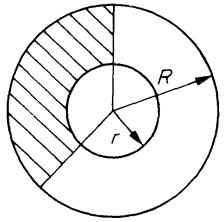
\includegraphics[width=0.2\textwidth]{img/d_algo.png}
\end{frame}

\begin{frame}
  \frametitle{Tsiligirides' Route-Improvement Algorithmus (RI)}
  \begin{itemize}
    \item Verbesserungsverfahren für initiale Routen (aus S-/D-Algorithmus)
    \item \textbf{3 Schritte}:
    \begin{itemize}
      \item Tausche Position zweier Knoten innerhalb der Route
      \begin{itemize}
        \item Reihenfolge der Knoten dazwischen bleibt gleich
        \item Reihenfolge der Knoten dazwischen wird umgekehrt
      \end{itemize}
      \item Pot. Erweiterung der Route durch unbesuchte Knoten
      \item Ersetze besuchte durch besser geeignete unbesuchte Knoten
    \end{itemize}
    \item Sämtliche Schritte werden nur ausgeführt, wenn der \textit{profit} verbessert und $T_{max}$ eingehalten wird
    \item Knoten werden stets an der günstigsten Stelle eingefügt
  \end{itemize}
\end{frame}

\begin{frame}
  \frametitle{Center-of-Gravity Heuristik}
  \textbf{Idee:}
  Verbesserung der Route durch Einfügen von Knoten mit hohem Score \textquote{in der Mitte der Route}\

  \textbf{3 Schritte:}
  \begin{enumerate}
    \item Konstruktion der Route
    \item Verbesserung der Route
    \item Iterative Verbesserung durch Center-of-Gravity-Verfahren
  \end{enumerate}
  Die ersten beiden Schritte werden verwendet, um eine initiale Route zu generieren.
\end{frame}

\begin{frame}
  \frametitle{1.) Konstruktion der Route}
  \begin{itemize}
    \item \textbf{Ziel}:\newline Route generieren, die mit $1$ startet, mit $n$ endet, einen möglichst hohen \textit{profit} besitzt
    und $\leq T_{max}$ Zeit benötigt
    \item \textbf{Einfügeheuristik}:\newline
    Idee: Knoten einfügen, die einen großen \textit{score} haben und der Route
    möglichst wenig zusätzliche \textit{travel costs} hinzufügen\newline
    $\rightarrow$ möglichst große $\frac{P_j}{t_{lj}}$
  \end{itemize}
\end{frame}

\begin{frame}
  \frametitle{2.) Verbesserung der Route}
  \begin{itemize}
    \item Bekommt die zuvor generierte Route als Input
    \item Verwendet eine Austauschprozedur wie \textsc{2-OPT}, um eine kürzere Route für dieselbe Knotenmenge zu finden
    \item Anschließend wird \textquote{Cheapest-Insertion} verwendet, wobei der der Route so viele Knoten wie möglich hinzugefügt werden,
    ohne $T_{max}$ zu verletzen
  \end{itemize}
\end{frame}

\begin{frame}
  \frametitle{3.) Center-of-Gravity}
  \textbf{Idee:} Berechne gewichtetes Zentrum der Route.\newline

  Angenommen, Knoten $i$ besitzt die Koordinaten $x(i), y(i)$\newline

  \textbf{Center of Gravity} $g = (\bar{x}, \bar{y})$ mit:\newline

  $\bar{x} = \frac{\sum_{i \in L} P_i x(i)}{\sum_{i \in L} P_i} \quad\quad
  \bar{y} = \frac{\sum_{i \in L} P_i y(i)}{\sum_{i \in L} P_i}$\newline

  Berechne $\frac{P_i}{t_{ig}}$ für $i = 1, 2, ..., n$\newline

  Intuition: Wir wollen profitable Knoten, die nah am CoG liegen.
\end{frame}

\begin{frame}
  \frametitle{3.) Center-of-Gravity}
  \textbf{Anschließend wird die Route wie folgt verbessert:}
  \begin{itemize}
    \item \textit{Cheapest-Insertion} in abst. Reihenfolge $\frac{P_i}{t_{ig}}$ solange $T_{max}$ eingehalten wird
    \item Erneute Verbesserung der Route (Schritt 2)
  \end{itemize}
  \textbf{Bestimmung einer Lösung}:
  \begin{itemize}
    \item Wiederholter Center-of-Gravity-Schritt für Lösungsroute
    \item Iterativer Prozess, bis Konvergenz erreicht ist
    \item Beste generierte Route wird ausgewählt
  \end{itemize}
\end{frame}

\begin{frame}
  \frametitle{Local Search Moves}
  \textbf{$2$ Arten: Moves, die...}
  \begin{itemize}
    \item ... die \textit{travel costs} für eine Teilmenge der Knoten verringern
    \item ... den \textit{profit} durch eine verbesserte Knotenauswahl erhöhen
  \end{itemize}
  Die Operatoren sollten nur angewandt werden, wenn die Route verbessert und weiterhin zulässig ist.
\end{frame}

\begin{frame}
  \frametitle{Local Search Moves}
  \textbf{Verringerung der \textit{travel costs}:}
  \begin{itemize}
    \item \textsc{SWAP}: Tausche zwei Knoten innerhalb einer Route
    \item \textsc{RELOCATE}: Ändere Pos. eines Knotens in einer Route
    \item \textsc{2-OPT}: Ersetze zwei Kanten einer Route durch zwei andere
  \end{itemize}
\end{frame}

\begin{frame}
  \frametitle{Local Search Moves}
  \textbf{Steigerung des \textit{profits}:}
  \begin{itemize}
    \item \textsc{INSERT}: Füge der Route einen neuen Knoten hinzu (\textit{Cheapest-Insertion})
    \item \textsc{REPLACE}: Ersetze einen Knoten der Route durch einen nicht besuchten Knoten mit größerem \textit{profit}
  \end{itemize}
\end{frame}

\begin{frame}
  \frametitle{Particle Swarm Optimization (PSO)}
  \begin{itemize}
    \item Populations-basierter stochastischer Optimierungsalgorithmus
    \item Inspiriert durch intelligentes kollektives Verhalten best. Tiere
    \item Kooperative Art, Futter zu finden (Zielfkt. zu optimieren)
    \item Balance zwischen \textit{Exploration} und \textit{Exploitation}
  \end{itemize}
  \begin{figure}
    \centering
    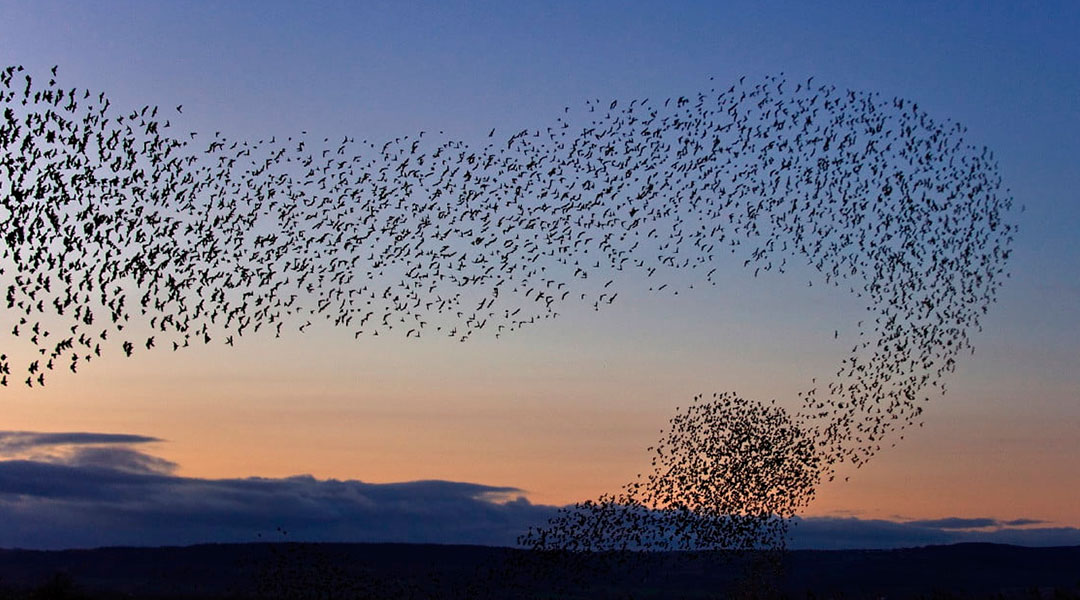
\includegraphics[width=0.75\textwidth]{img/birds.jpg}
  \end{figure}
\end{frame}

\begin{frame}
  \frametitle{Particle Swarm Optimization (PSO)}
  \begin{figure}
    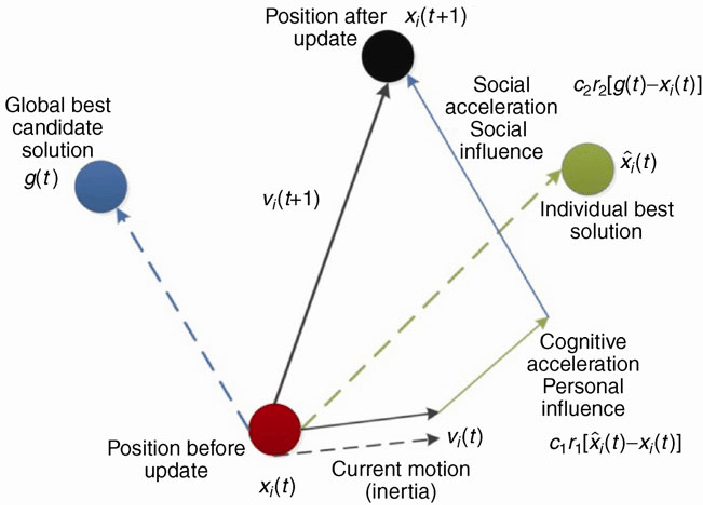
\includegraphics[width=0.7\textwidth]{img/PSO.png}
  \caption*{Particle Position Update}
  \end{figure}
\end{frame}

\begin{frame}
  \frametitle{Particle Swarm Optimization (PSO)}
  \textbf{Nachteile}:
  \begin{itemize}
    \item \textquote{Premature Convergence}
    \item Fehlende Intensivierung um lokale Optima
  \end{itemize}
  \textbf{Maßnahmen zur Verbesserung}:
  \begin{itemize}
    \item Geschwindigkeit der wegweisenden Partikel wird zufällig aktualisiert \textrightarrow verbessert
    \textquote{Exploration} und verhindert \textquote{Premature Convergence}
    \item Verbesserung der \textquote{Exploitation-Fähigkeit} der wegweisenden Partikel durch RVNS
  \end{itemize}
\end{frame}

\begin{frame}
  \frametitle{Adaptive Large Neighborhood Search (ALNS)}
  \textbf{Initiale Lösung}:
  \begin{itemize}
    \item Clustering nah beieinander liegender Knoten (\textsc{DBSCAN})
    \item Knoten werden randomisiert nacheinander in die Route einfügt solange keine NB verletzt wird
    \item Knoten desselben Clusters werden mit höherer Wahrscheinlichkeit ausgewählt
  \end{itemize}
\end{frame}

\begin{frame}
  \frametitle{Adaptive Large Neighborhood Search (ALNS)}
  \textbf{Verbesserung der Lösung}:
  \begin{itemize}
    \item \textbf{destroy}:
    \begin{itemize}
      \item \textsc{RANDOM REMOVE}
      \item \textsc{RANDOM SEQUENCE REMOVE}
      \item \textsc{RANDOM CLUSTER REMOVE}
    \end{itemize}
    \item \textbf{repair}: 
    \begin{itemize}
      \item \textsc{GREEDY REPAIR}
      \item \textsc{RANDOM REPAIR}
      \item \textsc{PRIZE REPAIR}
      \item \textsc{CLUSTER REPAIR}
    \end{itemize}
  \end{itemize}
\end{frame}

\end{document}
